\begin{frame}{Anstandsjagt}
    
     \begin{columns}[T]
        \begin{column}{0.58\textwidth}
            \begin{itemize}
                \item \textbf{Passiv} jagtform – jægeren venter på vildtet
                \item Jægeren placerer sig strategisk i terrænet
                \item Foregår typisk fra: jagttårn, jagtstige, treestand
                \item Fordele:
                  \begin{itemize}
                    \item Kontrolleret og sikkert skud
                    \item God styr på vindretning
                    \item Vildtet forstyrres minimalt
                  \end{itemize}
                \item Vildtet drives ikke frem – det kommer naturligt
                \item Meget udbredt på hjortevildt (råvildt, dåvildt, kronvildt)
                \item Kræver tålmodighed, god placering og viden om vildtets færden
                \item Anvendes ikke hunde til denne jagtform
            \end{itemize}
        \end{column}
        
         \begin{column}{0.4\textwidth}
            \centering
            \vspace{0.5em}
            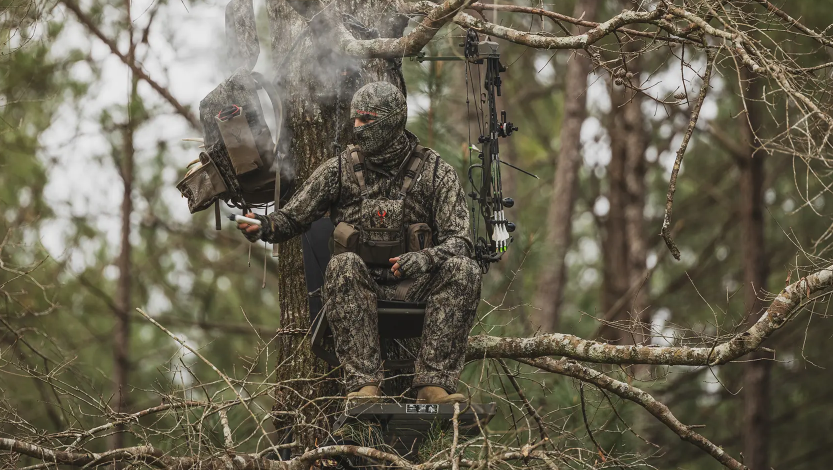
\includegraphics[width=\textwidth,height=0.82\textheight,keepaspectratio]
                {Billeder/Jagtformer/anstandsjagt.png}
            % Alternativer – fjern kommentartegn hvis du vil skifte:
            % \includegraphics[width=\textwidth]{highseat-snow-forest-hunter.jpg}
            % \includegraphics[width=\textwidth]{hunter-highseat-morning-mist.jpg}
            % \includegraphics[width=\textwidth]{ansitz-jagttarn-skov.jpg}
        \end{column}
    \end{columns}
    
\end{frame}